\documentclass[11pt,a4paper]{article}
\usepackage[margin=21mm,top=20mm,bottom=22mm]{geometry}
\usepackage{lmodern}
\usepackage[T1]{fontenc}
\usepackage{microtype}
\usepackage{amsmath,amssymb}
\usepackage{booktabs,tabularx,array,longtable}
\usepackage{graphicx,xcolor,float}
\usepackage[font=small,labelformat=empty,skip=4pt]{caption}
\usepackage{enumitem}
\usepackage[hidelinks]{hyperref}
\usepackage{titlesec}
\definecolor{ink}{HTML}{1B2430}\definecolor{quote}{HTML}{5B6673}
\titleformat{\section}{\large\bfseries\color{ink}}{\thesection}{0.7em}{}
\titleformat{\subsection}{\normalsize\bfseries\color{ink}}{\thesubsection}{0.6em}{}
\titlespacing*{\section}{0pt}{16pt}{6pt}\titlespacing*{\subsection}{0pt}{12pt}{4pt}
\newcommand{\paper}[1]{{\color{quote}\itshape #1}}
\newcommand{\note}[1]{{\color{quote}\itshape (#1)}}
\newcommand{\fup}{the follow-up paper \href{https://arxiv.org/abs/2403.10772}{[arXiv:2403.10772]}}
\newcommand{\fupc}{the code released with \href{https://arxiv.org/abs/2403.10772}{[arXiv:2403.10772]}}
\newcommand{\cur}{the current code of \href{https://arxiv.org/abs/2505.19332}{[arXiv:2505.19332]}}
\newcommand{\meth}{the earlier method paper \href{https://arxiv.org/abs/2103.11484}{[arXiv:2103.11484]}}
\newcolumntype{Y}{>{\raggedright\arraybackslash}X}
\newcolumntype{P}[1]{>{\raggedright\arraybackslash}p{#1}}
\linespread{1.18}
\setlength{\parskip}{7pt}\setlength{\parindent}{0pt}\setlength{\emergencystretch}{2.5em}
\renewcommand{\arraystretch}{1.28}
\setlength{\tabcolsep}{5pt}
\captionsetup[table]{labelformat=simple,labelfont=bf,skip=6pt}
\begin{document}

{\LARGE\bfseries Reproduction of arXiv:2309.12402 with SDPB}\\[4pt]
{\large A comparison with the figures of the paper}\\[8pt]
{Bo Wang, Shi Qiu, Hua Xing Zhu}\\[2pt]
{\color{quote}14 September 2026}
\vspace{6pt}\hrule\vspace{8pt}

\section{What was done}
This note compares our reproduction of the finite S-matrix / form-factor bootstrap of \emph{Bootstrapping gauge theories} \note{arXiv:2309.12402, version 3} with the figures of that paper.

The optimisation was carried out with SDPB 3.1.0 \note{192-bit arithmetic, duality-gap threshold $10^{-6}$, primal and dual error thresholds $10^{-10}$}, with the finite problem written directly as a polynomial-matrix program. No other solver was used at any stage.

The discretised operators were derived from Sections~2 and~3 of the paper \note{the conformal map and collocation grid (3.58)--(3.62), the cot kernel (3.67), the angular projections of the Mandelstam representation (2.7), and the current kernels (3.68)--(3.75)} and were checked in three independent ways: a Mathematica script recomputes the formulas at $M=50$, an independent reconstruction of the (2.7) projections agrees with the production operators to $5\times10^{-15}$ over all 3876 coefficients, and every accepted solution is re-verified against all of the original constraints in Arb interval arithmetic.

Table~\ref{tab:inputs} collects the inputs we took as printed. Five numerical choices are not specified in the paper and turn out to decide the outcome for Figures~8--10; Table~\ref{tab:open} lists them together with the readings we ran.

\begin{table}[H]\small
\caption{Inputs taken as printed in the paper.}\label{tab:inputs}
\begin{tabularx}{\textwidth}{@{}P{0.30\textwidth}Y@{}}
\toprule
Discretisation & $M=50$, $\phi_i=(i-\tfrac12)\pi/M$, $\nu_0=0$; unitarity imposed for $L=10$ waves per isospin \\
Matching scale and QCD inputs & $s_0=(1.2\,\text{GeV})^2$, $\alpha_s=0.4$, $m_u=4$\,MeV, $m_d=7.3$\,MeV, the condensates of (2.54), $m_\pi=140$\,MeV, $f_\pi=92$\,MeV \\
Sum rules & the printed numbers of (2.56) times $s_0^{\,n+2}$; moments $n=0,1$ for S0 and $n=-1,0$ for P1; $\epsilon^{SR}=2\times10^{-3}$ \\
Form factors & $\epsilon^{FF}=6\times10^{-5}$ in (3.75) \\
Chiral matching & points $s=\tfrac12,1,\tfrac32,2$; $\epsilon^\chi=2\times10^{-3}$ \\
\bottomrule
\end{tabularx}
\end{table}

\begin{table}[H]\small
\caption{Choices the paper leaves unspecified, and the readings we ran.}\label{tab:open}
\begin{tabularx}{\textwidth}{@{}P{0.26\textwidth}P{0.25\textwidth}Y@{}}
\toprule
Item & Paper text & Readings run \\
\midrule
Norm of the sum-rule tolerance (3.73), $\epsilon^{SR}=2\times10^{-3}$ & \paper{with some norm} & a per-moment box on the raw moments \note{main line}; a per-wave $L^2$ ball \note{the structure used in \fupc}; a relative 10\,\% box per moment \\
\addlinespace
Evaluation point of the factor between $F$ and $\mathcal F$ in (3.75) & \paper{which we evaluate at $s=s_0$} \note{in the estimate of $\epsilon^{FF}$} & the factor at each node $s_i>s_0$ \note{main line}; the factor frozen at $s_0$ \\
\addlinespace
Regularisation of the double spectral density & not mentioned in the paper; \meth, Section~3, and \fupc\ use an $M$-bound & $|\rho_{ij}|\le M_{\rm reg}$, with $M_{\rm reg}$ fixed by an in-model rule \note{omitted-wave unitarity and $L$-stability}: $10^2$ for the chiral and UV stages, $10^3$ for the pure stage; $\ell^2$, $\ell^4$ and $M_{\rm reg}\times10$ controls \\
\addlinespace
Amplitude at a boundary point & \paper{only points at the boundary have partial waves associated with them} & the solver's optimal point, together with a diagnostic of the whole near-optimal face \note{Section~4} \\
\addlinespace
Chiral norm in (3.64) & \paper{with some norm} & one combined 8-dimensional $L^2$ norm \note{as in \fupc}; two separate 4-dimensional norms as a control \\
\bottomrule
\end{tabularx}
\end{table}

\section{Summary}
\begin{table}[H]\small
\caption{Figure-by-figure summary; the details and the side-by-side figures follow in Section~3.}\label{tab:summary}
\begin{tabularx}{\textwidth}{@{}lP{0.23\textwidth}YP{0.21\textwidth}@{}}
\toprule
Figure & Paper statement & Our result & Agreement \\
\midrule

Fig.~3 & pure-unitarity region, $M=50$, $L=10$ & $+x$ end 2.22445 vs 2.23289 (\ensuremath{-0.4\,\%}); $-x$ end \ensuremath{-2.247} vs \ensuremath{-2.902}; $f_1^1$ range $[\ensuremath{-0.6243},0.06629]$ vs $[\ensuremath{-0.7336},0.07932]$ & the $+x$ end agrees; our region lies inside yours on the $-x$ and $\pm y$ sides \\\addlinespace
Fig.~4 & the chiral constraints collapse the region onto $f_1^1=-f_0^0/15$ & $\epsilon^\chi=2\times10^{-3}$: $+x$ end 0.082757 vs 0.0825728 (\ensuremath{+0.2\,\%}); $x_{\rm ref}$ section width \ensuremath{7.618\times10^{-4}} vs \ensuremath{7.598\times10^{-4}}; the six-tolerance ladder is monotone & agrees \\\addlinespace
Fig.~5 & the subthreshold waves are nearly linear and the S0 chiral zero moves with $\epsilon^\chi$ & RMS $\le 6.4\,\%$ of $f_0^0(3)$ against the digitised curves at $\epsilon^\chi=2,4,6\times10^{-3}$; S0 zero at $s=0.426$, $0.293$, absent & agrees \\\addlinespace
Fig.~7 & with the chiral constraints alone S0 and S2 agree with experiment and P1 has no $\rho$ & RMS against the digitised curves S0 0.388$^\circ$, S2 0.144$^\circ$, P1 0.456$^\circ$; no P1 crossing below 1.2\,GeV & agrees \\\addlinespace
Fig.~8 & with the sum rules the upper boundary shrinks much more than the lower one & upper shrink / lower rise at $x_{\rm ref}$: \ensuremath{2.8\times10^{-4}} / \ensuremath{2.8\times10^{-4}} (factor at each node), \ensuremath{5.3\times10^{-5}} / \ensuremath{2.5\times10^{-4}} (factor frozen at $s_0$); paper $2.32\times10^{-4}$ / $3.7\times10^{-5}$. $+x$ end 0.076013 / 0.079623 vs 0.08112 & the asymmetry does not appear in any feasible reading \\\addlinespace
Fig.~9 & P1 phase shift with the $\rho$; the 90$^\circ$ crossing lies about 6\,\% above 770\,MeV & crossings: tip 772.7\,MeV ($|S|_{\min}=0.585$), mid 738.9\,MeV ($|S|_{\min}=0.077$); at the reference point $|S|$ dips to 0.24 at 0.73\,GeV (708\,MeV on the $+180^\circ$ branch); paper 813--827\,MeV & a $\rho$-like structure appears at every point once the UV constraints are added; it lies 40--110\,MeV below yours and is strongly inelastic \\\addlinespace
Fig.~10 & S0 and S2 coincide at low energy and spread above & S2: RMS 0.354--1.44$^\circ$, endpoints $-28$ to $-32^\circ$ (paper $-18$ to $-36^\circ$); S0: RMS 5.7--16.6$^\circ$, endpoint at 1.196\,GeV 181--192$^\circ$ (paper 87--106$^\circ$) & S2 agrees; S0 rises faster than yours above 0.6\,GeV \\\addlinespace
Fig.~11 & good convergence in $L$; the $\rho$ peak shifts with $M$ & P1 crossing at $M=50$, $L=8/10/12$: 771.4 / 772.7 / 772.9\,MeV; $L=10$, $M=45/50/60$: 736.1 / 772.7 / 738.8\,MeV; S0 at 1\,GeV 150--165$^\circ$ (paper about 95$^\circ$) & the $L$ dependence agrees; the shift with $M$ is 37\,MeV; the S0 level differs \\\addlinespace
\bottomrule
\end{tabularx}
\end{table}

\section{Figure-by-figure comparison}
For each figure, the panel on the left (or top) reproduces the figure from the arXiv source of the paper, and the panel on the right (or bottom) shows our accepted solutions together with the digitised curve or boundary from the paper. Quotations from the paper are set in \paper{grey italics}.

\subsection{Fig.~3, pure unitarity region}
\paper{``we have used $M=50$ in (3.61) for discretization and imposed unitarity for 10 partial waves per isospin.''}

We computed 24 support directions in steps of 15$^\circ$, all of which were accepted, at $M=50$, $L=10$ and $M_{\rm reg}=10^3$ \note{at this scale the six lowest omitted waves stay within $|S|\le1.02$ at every node and the $L=8/10/12$ endpoints agree to 2\,\%}. Against the digitised figure the extrema are $f_0^0$ max 2.22445 vs 2.23289 (\ensuremath{-0.4\,\%}), $f_0^0$ min \ensuremath{-2.247} vs \ensuremath{-2.902}, $f_1^1$ min \ensuremath{-0.6243} vs \ensuremath{-0.7336} and $f_1^1$ max 0.06629 vs 0.07932. The $+x$ end hardly depends on $M_{\rm reg}$ (2.2116, 2.2245 and 2.2305 at $10^2$, $10^3$ and $10^4$), whereas the other three extrema lie inside your region by 15--23\,\%; these are the directions in which the amplitudes are largest and the $|\rho_{ij}|$ bound is active, so we regard them as measuring the unspecified regulariser rather than the model itself. A control at $M_{\rm reg}=10^4$ for these three directions is still running.

\begin{figure}[H]\centering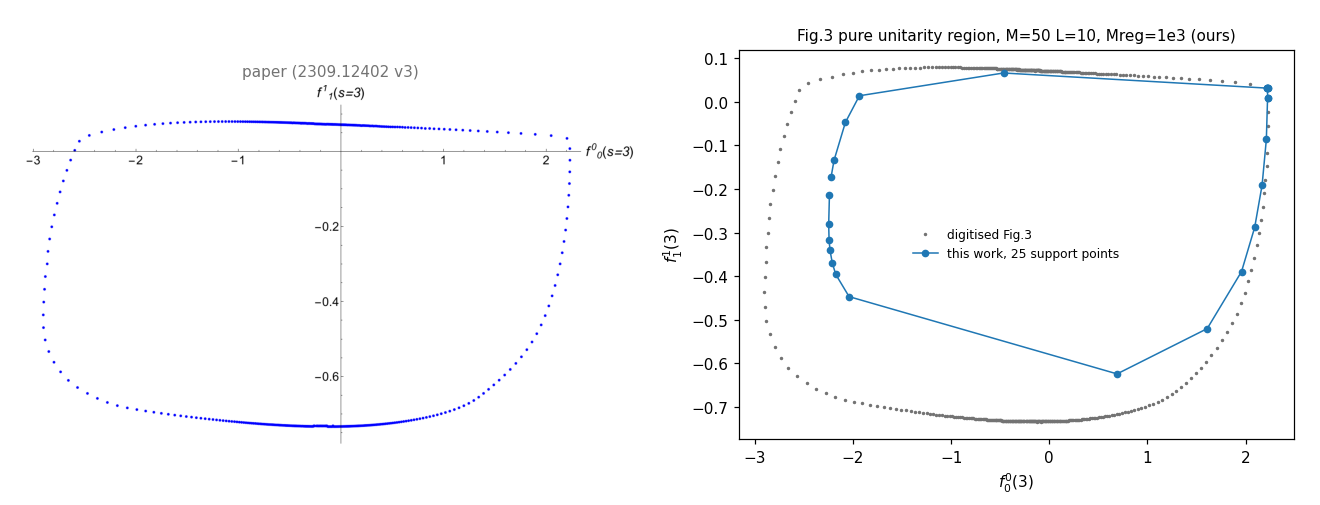
\includegraphics[width=\textwidth]{figures/fig3.png}\caption{Fig.~3: the paper (left) and our 24 support points with the digitised boundary (right).}\end{figure}

\subsection{Fig.~4, chiral constraints}
\paper{``restricted by the chiral constraints (3.64) with tolerances $6\times10^{-3}$, $4\times10^{-3}$, $2\times10^{-3}$, $1\times10^{-3}$, $6\times10^{-4}$, $2\times10^{-4}$ (from the outer shape inward) \dots\ with some norm''}

The chiral constraints are imposed as one combined 8-dimensional $L^2$ norm on the four-point residuals, the packaging used in \fupc, with $M_{\rm reg}=10^2$. At $\epsilon^\chi=2\times10^{-3}$ the $+x$ end is 0.082757 (paper 0.0825728, \ensuremath{+0.2\,\%}) and the vertical section at $x_{\rm ref}$ has width \ensuremath{7.618\times10^{-4}} (paper \ensuremath{7.598\times10^{-4}}); the $+x$ ends of the six tolerances decrease monotonically, 0.1608, 0.1255, 0.0828, 0.0551, 0.0411, 0.0223 for $\epsilon^\chi=6\times10^{-3}$ down to $2\times10^{-4}$. A control with two separate 4-dimensional norms moves the $+x$ end by less than the spacing of this ladder.

\begin{figure}[H]\centering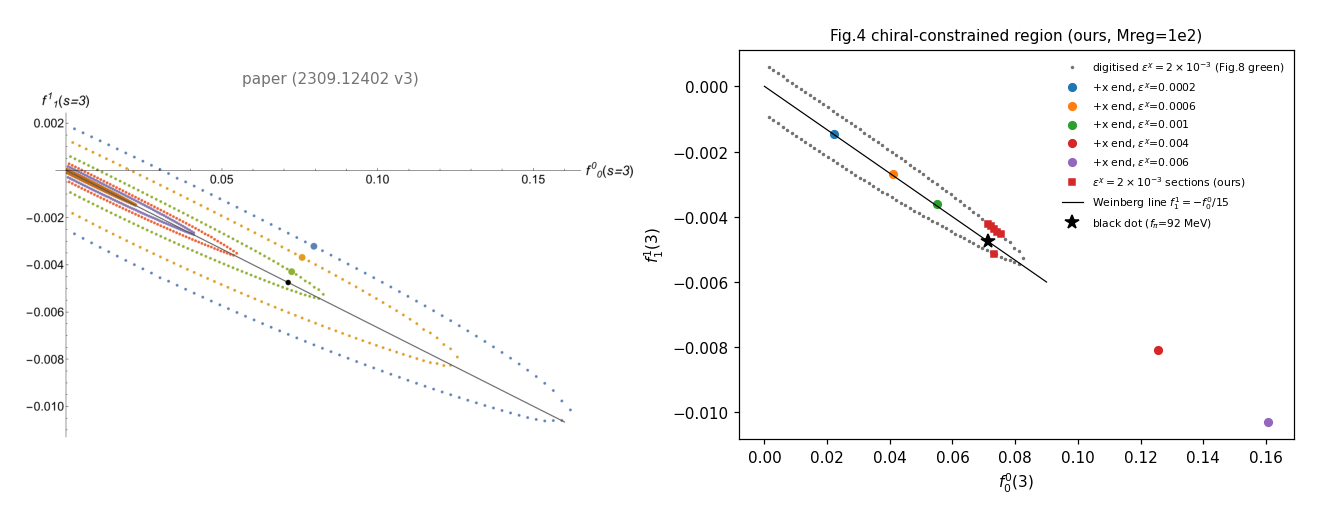
\includegraphics[width=\textwidth]{figures/fig4.png}\caption{Fig.~4: the paper (left); our six $+x$ ends and the $\epsilon^\chi=2\times10^{-3}$ sections, with the digitised $\epsilon^\chi=2\times10^{-3}$ boundary (right).}\end{figure}

\subsection{Fig.~5, subthreshold partial waves}
\paper{``For the larger tolerances the partial waves are not approximately linear \dots\ the chiral zero of the amplitude disappears for the blue points. \dots\ The value $\epsilon^\chi=0.002$ \dots\ allows the physical value of $f_\pi$.''}

The subthreshold curves are evaluated from the Arb coefficients of the accepted solutions on $0.05\le s\le3.95$, at the upper-branch $x_{\rm ref}$ representative of each tolerance. Their RMS deviation from your digitised curves is at most 6.4\,\% of $f_0^0(3)$, and the S0 zero sits at $s=0.426$ for $2\times10^{-3}$, at $0.293$ for $4\times10^{-3}$, and is absent at $6\times10^{-3}$, as in the figure.

\begin{figure}[H]\centering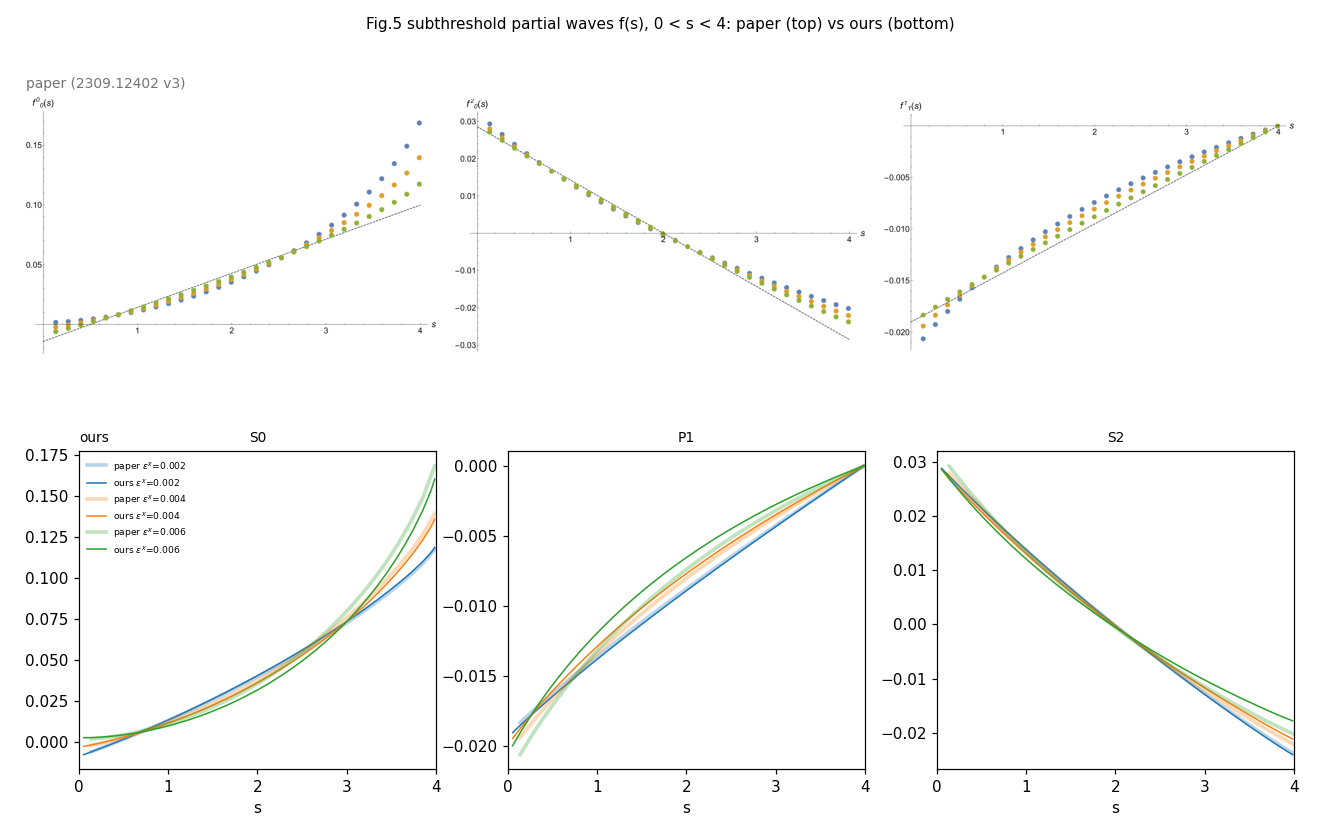
\includegraphics[width=\textwidth]{figures/fig5.png}\caption{Fig.~5: the three panels of the paper (top) and ours (bottom).}\end{figure}

\subsection{Fig.~7, chiral-only phase shifts}
\paper{``We choose a point closest to the black dot \dots\ The partial waves at the magenta point and other nearby agree very well with experimental values for the S0 and S2 waves but not for the P1.''}

The representative point was fixed by a rule chosen before any phase shift was read: among the upper-branch endpoints of the vertical sections at $x_{\rm ref}+\{-0.002,-0.001,0,+0.001,+0.002\}$ we take the one nearest to the black dot. The RMS deviations from your digitised curves are S0 0.388$^\circ$, S2 0.144$^\circ$ and P1 0.456$^\circ$, and P1 shows no 90$^\circ$ crossing below 1.2\,GeV.

\begin{figure}[H]\centering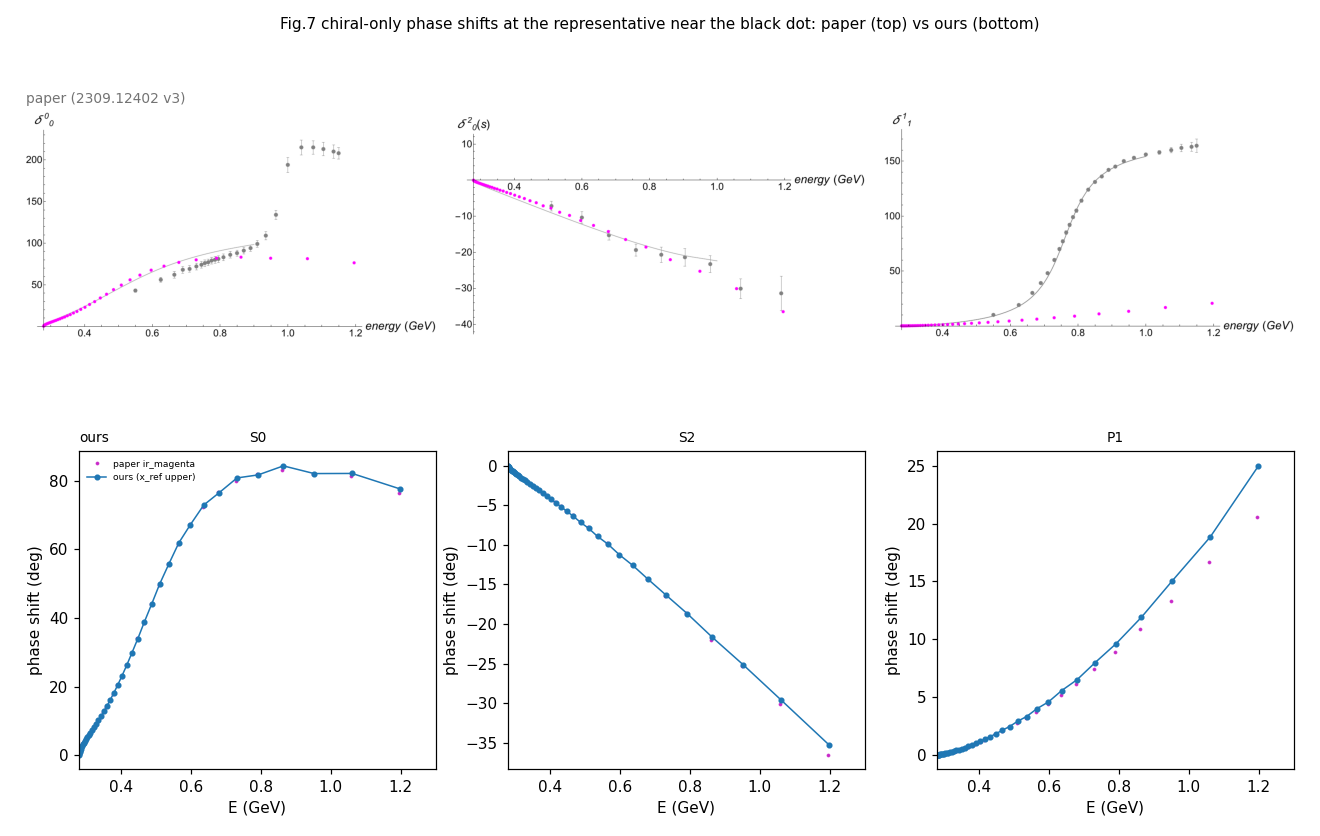
\includegraphics[width=\textwidth]{figures/fig7.png}\caption{Fig.~7: the paper (top) and ours (bottom).}\end{figure}

\subsection{Fig.~8, the region after the sum rules and the form-factor bounds}
\paper{``the plots are produced by taking $\epsilon^{SR}=2\times10^{-3}$ in (3.73) and $\epsilon^{FF}=6\times10^{-5}$''}; caption: \paper{``The upper boundary shrinks notable but the lower not so much.''}

We ran three readings of $\epsilon^{SR}$ and two of the (3.75) factor. The table gives the values at the $x_{\rm ref}$ section, with the paper values read from the digitised figure.

\begin{table}[H]\small\begin{tabularx}{\textwidth}{@{}Yrrrr@{}}\toprule Reading & UV $+x$ end & upper shrink & lower rise & ratio \\\midrule
raw box $2\times10^{-3}$ per moment, factor at each node & 0.076013 & \ensuremath{2.8\times10^{-4}} & \ensuremath{2.8\times10^{-4}} & 1 \\
raw box, factor frozen at $s_0$ & 0.079623 & \ensuremath{5.3\times10^{-5}} & \ensuremath{2.5\times10^{-4}} & 0.214 \\
per-wave $L^2$ ball $2\times10^{-3}$, factor frozen at $s_0$ & 0.079541 & \ensuremath{5.3\times10^{-5}} & \ensuremath{2.5\times10^{-4}} & 0.214 \\
paper (digitised) & 0.08112 & $2.32\times10^{-4}$ & $3.7\times10^{-5}$ & 6.3 \\\bottomrule\end{tabularx}\end{table}

The relative reading, 10\,\% of each moment, turned out to be infeasible in this model. To establish this we removed the box on the S0 $n=0$ moment, kept the other three 10\,\% boxes and every other constraint, and minimised that moment; the minimum is \ensuremath{3.745\times10^{-3}}, 1.57 times the QCD value, so no point of the feasible set lies within 10\,\% of it. In the raw-box reading the accepted solutions sit at the upper edge of three of the four boxes (S0 $n=0$ at $+84\,\%$ of its target, S0 $n=1$ at $+1.8\,\%$, P1 $n=0$ at $+1.4\,\%$), which shows that the sum rules do bind, in the direction of larger spectral integrals.

\begin{figure}[H]\centering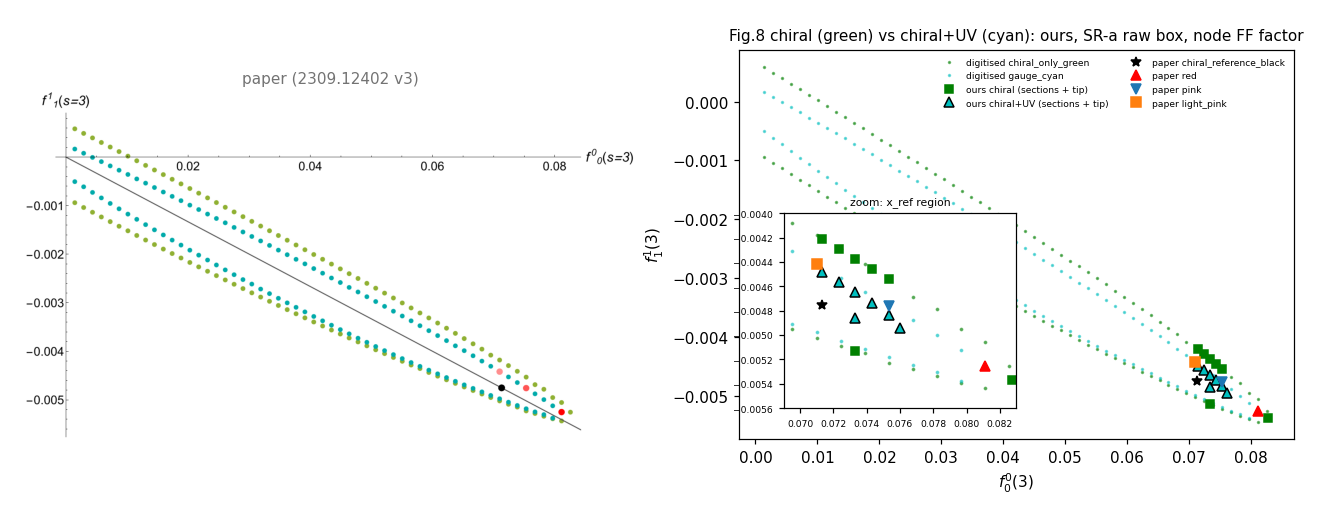
\includegraphics[width=\textwidth]{figures/fig8.png}\caption{Fig.~8: the paper (left); our chiral and chiral+UV boundary points with the digitised boundaries, and a zoom on the $x_{\rm ref}$ region (right).}\end{figure}

\subsection{Fig.~9, P1 phase shift}
\paper{``The resonance energy where the phase shift crosses $\pi/2$ is slightly shifted from the real world data on the mass of the rho at 770 MeV by roughly 6\,\%.''} The digitised crossings are at 0.827, 0.824 and 0.813\,GeV.

At the three representatives of the same frozen rule (the tip is the $+x$ end, the reference point is the upper-branch point nearest to the black dot, and the mid point is its neighbour towards the tip) we find the following. At the tip the phase crosses 90$^\circ$ at 772.7\,MeV with $|S_{P1}|=0.585$ at 0.79\,GeV; at the mid point it crosses at 738.9\,MeV with $|S_{P1}|$ dropping to 0.077; at the reference point $|S_{P1}|$ falls to 0.24 at 0.73\,GeV and the node values admit two phase branches, the nearest-node lift swinging to $-47^\circ$ while the $+180^\circ$ branch crosses 90$^\circ$ at 708\,MeV. Since the chiral constraints alone (Fig.~7) give no crossing below 1.2\,GeV, the resonance is produced by the sum rules and the form-factor bounds, as in the paper; it appears 40--110\,MeV below yours and the wave is far from elastic there. The paper does not show $|S|$, which we add in the second panel.

\begin{figure}[H]\centering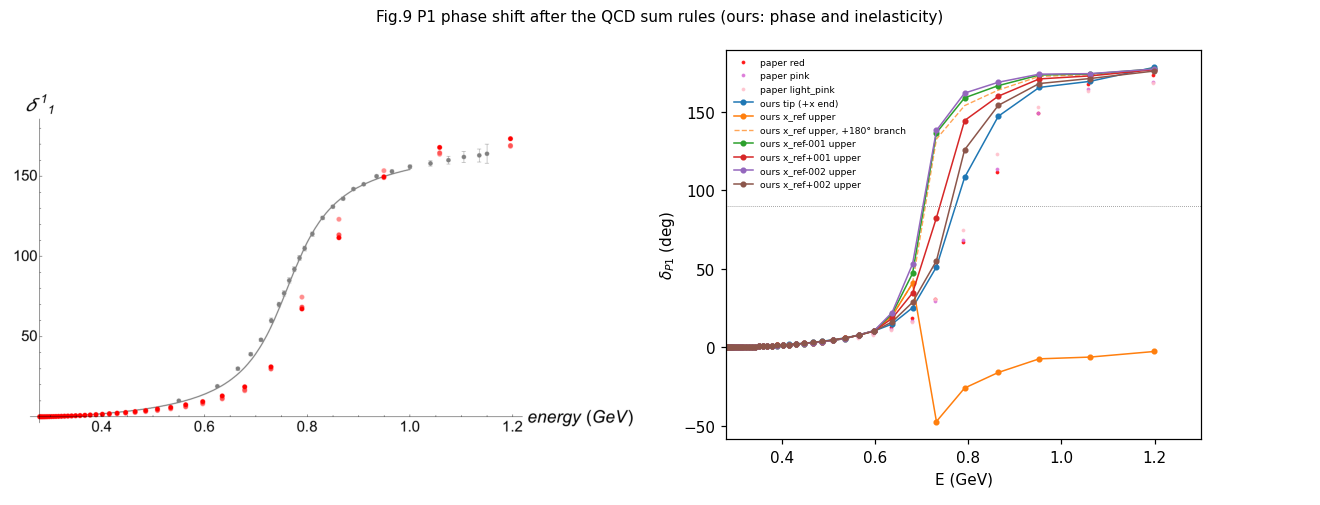
\includegraphics[width=\textwidth]{figures/fig9.png}\caption{Fig.~9: the paper (left) and our P1 phases at the representatives, with the three digitised curves (right).}\end{figure}
\begin{figure}[H]\centering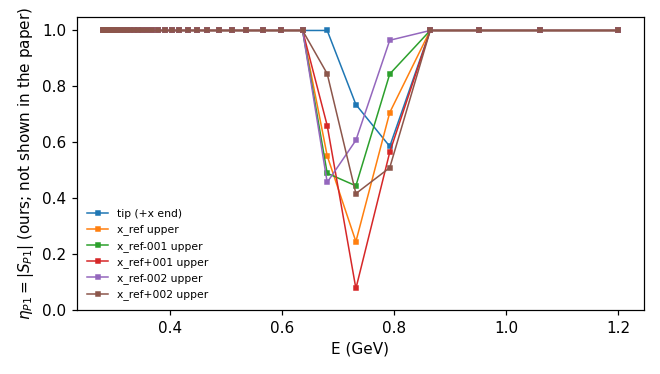
\includegraphics[width=0.62\textwidth]{figures/fig9_eta.png}\caption{$|S_{P1}|$ at the same points (not shown in the paper).}\end{figure}

\subsection{Fig.~10, S0 and S2 phase shifts}
\paper{``the three bootstrap (red, pink, light pink) curves \dots\ coincide at low energy but they spread at high energy.''}

S2 agrees with your curves (RMS 0.354--1.44$^\circ$, endpoints $-28$ to $-32^\circ$ at 1.196\,GeV against your $-18$ to $-36^\circ$). S0 agrees below about 0.6\,GeV and then rises faster, crossing 90$^\circ$ at 0.69\,GeV and reaching 181--192$^\circ$ at 1.196\,GeV, where your curves are at 87--106$^\circ$; since with the chiral constraints alone our S0 matches your Fig.~7 to 0.4$^\circ$, this difference is introduced by the UV constraints.

\begin{figure}[H]\centering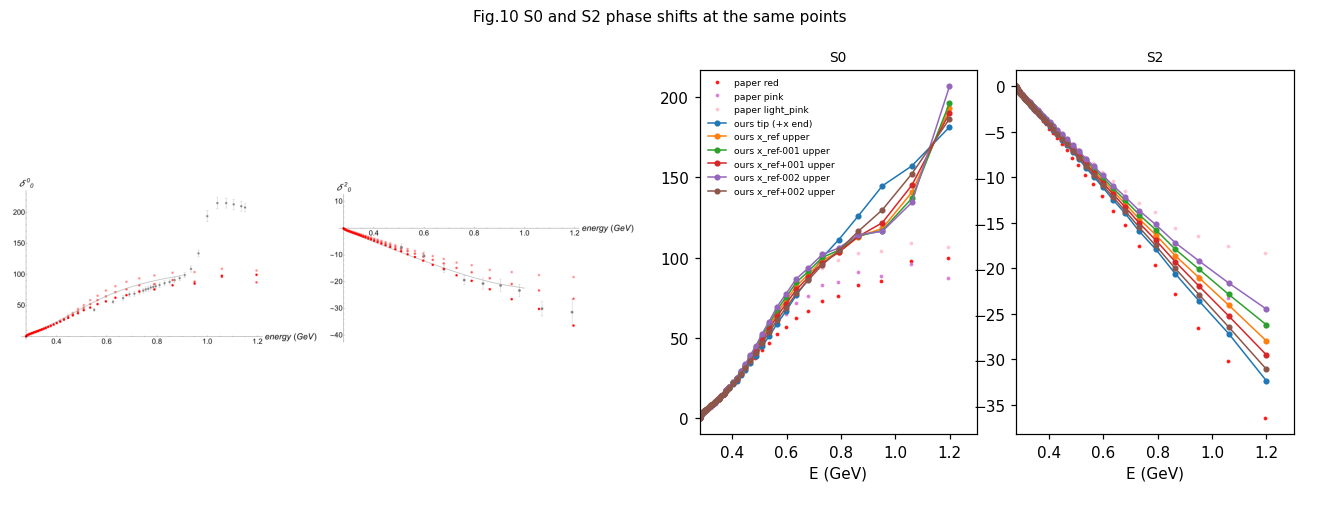
\includegraphics[width=\textwidth]{figures/fig10.png}\caption{Fig.~10: the paper (top) and ours (bottom).}\end{figure}

\subsection{Fig.~11, dependence on $M$ and $L$}
\paper{``For $M=50$, we have plotted the results with $L=8$, $10$, $12$. In all three partial waves there is a reasonably good convergence. \dots\ the P1 phase shifts show a $\rho$ resonance with the peak slightly shifted depending on $M$.''}

\begin{table}[H]\small\begin{tabularx}{\textwidth}{@{}lrrrr@{}}\toprule $(M,L)$ & UV $+x$ end & P1 crossing (MeV) & $\min|S_{P1}|$ below 1.2\,GeV & S0 at 1\,GeV ($^\circ$) \\\midrule

(50, 8) & 0.076176 & 771.4 & 0.584 & 151 \\
(50, 10) & 0.076013 & 772.7 & 0.585 & 150 \\
(50, 12) & 0.075944 & 772.9 & 0.585 & 150 \\
(45, 10) & 0.074275 & 736.1 & 0.226 & 165 \\
(60, 10) & 0.075097 & 738.8 & 0.597 & 156 \\
\bottomrule\end{tabularx}\end{table}

The $L$ dependence amounts to 1.5\,MeV in the crossing and 0.3\,\% in the endpoint. The $M$ dependence is 37\,MeV, with both $M=45$ and $M=60$ below $M=50$, whereas in your figure the ordering is $M=60<M=45<M=50$; the S0 level at 1\,GeV is 150--165$^\circ$ at every configuration, against about 95$^\circ$ in your figure.

\begin{figure}[H]\centering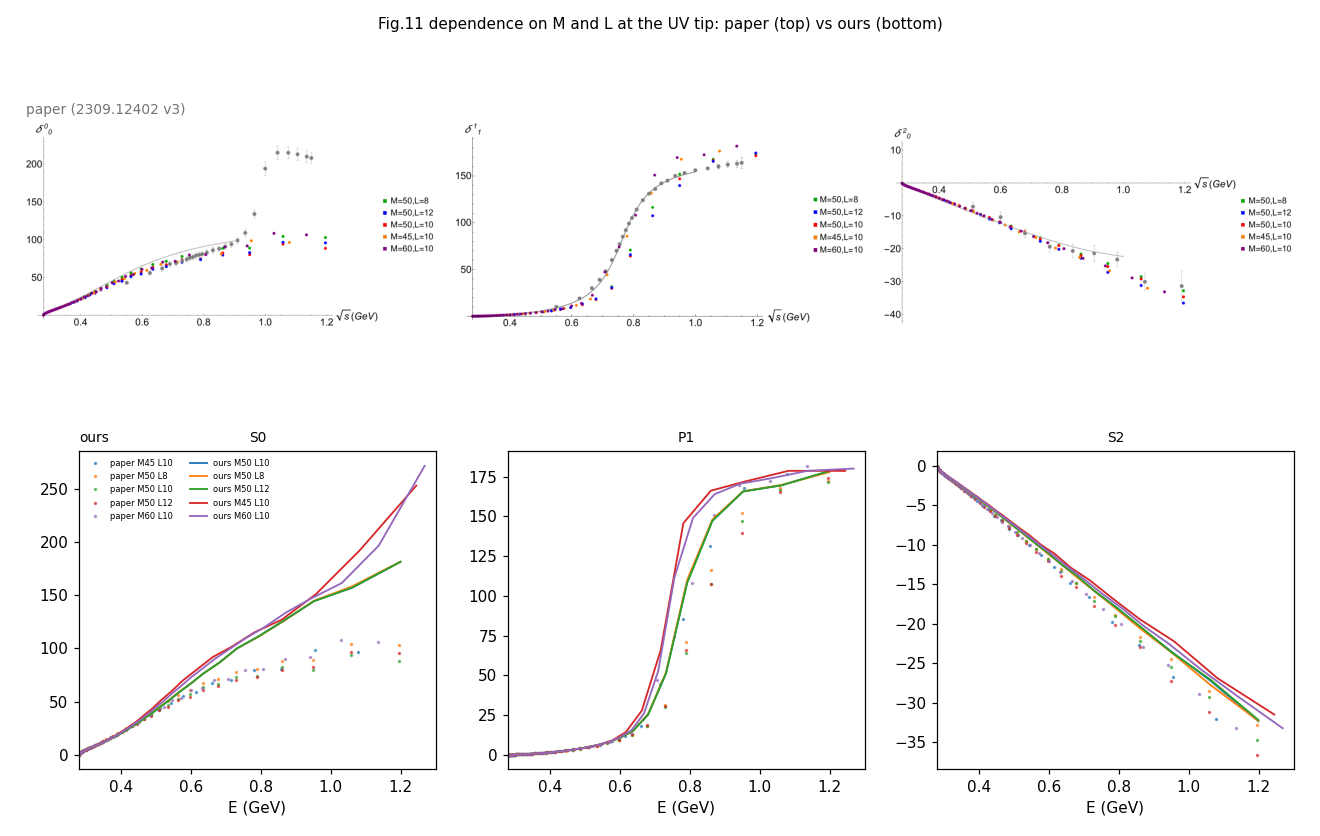
\includegraphics[width=\textwidth]{figures/fig11.png}\caption{Fig.~11: the paper (top) and ours (bottom).}\end{figure}

\section{Why the fine features of Figs.~8--10 do not follow from the stated problem}
Two diagnostics were applied to the accepted UV solutions, both exact up to the solver tolerance.

\textbf{Near-optimal face.} At a boundary point with support direction $d$ and optimal value $v^*$ we add the constraint $d\cdot(f_0^0,f_1^1)\ge v^*-2\times10^{-6}$ (twice the duality-gap threshold), keep the section, and maximise or minimise one node functional that is linear in the primal variables: $1-\operatorname{Re}S(s_i)$, $\operatorname{Im}S(s_i)$ or $\operatorname{Im}F(s_i)$. The range of the functional over this slab measures how far the amplitude at that boundary point is determined by the extremal problem. Your Fig.~9 phases at the nodes 0.792\,GeV (68.7--76.2$^\circ$) and 0.864\,GeV (112.8--124.1$^\circ$) have $\cos2\delta<0$, so an amplitude with those phases has $1-\operatorname{Re}S>1$ whatever the value of $|S|$.

\begin{table}[H]\small\begin{tabularx}{\textwidth}{@{}P{0.17\textwidth}P{0.2\textwidth}P{0.17\textwidth}Y@{}}\toprule Representative & Functional & Range over the face & Consequence \\\midrule
tip ($+x$ end) & $1-\operatorname{Re}S_{P1}$ (0.792\,GeV) & $[1.441,\,1.493]$ & pinned to $\pm0.03$ around the tip's own value 1.470, below the 1.72--1.85 of your curves at $|S|=1$ \\
tip & $1-\operatorname{Re}S_{P1}$ (0.864\,GeV) & $\le 0.6346$ & below 1: your 112.8--124.1$^\circ$ is excluded for every $|S|$ \\
tip & $\operatorname{Im}S_{P1}$ (0.792\,GeV) & $\le \ensuremath{-0.276}$ & negative on the whole face: every amplitude there is already past the resonance at 0.79\,GeV \\
$x_{\rm ref}$ upper (reference) & $1-\operatorname{Re}S_{P1}$ (0.792\,GeV) & $[0.02279,\,0.9356]$ & wide, hence undetermined, yet below 1 everywhere: your 68.7--76.2$^\circ$ is excluded for every $|S|$ \\
$x_{\rm ref}$ upper & $1-\operatorname{Re}S_{P1}$ (0.864\,GeV) & $\le 0.701$ & below 1: excluded for every $|S|$ \\
$x_{\rm ref}$ upper & $\operatorname{Im}F_1$ (0.792\,GeV) & $[0.07843,\,3.71]$ & the vector form factor is essentially free at this point \\
tip & $1-\operatorname{Re}S_{S0}$ (0.792\,GeV) & $[1.59,\,1.726]$ & the S0 phase is fixed at 111$^\circ$ on the face and only $|S|$ varies (0.79--0.99) \\\bottomrule\end{tabularx}\end{table}

The tip face is rigid in the P1 observables and does not contain your P1 shape. The $x_{\rm ref}$ face is degenerate, in the sense that a boundary point there does not carry a single set of partial waves, and it still excludes your P1 phase at both nodes. A different point on these faces, or a different solver, therefore cannot reproduce Fig.~9 from this constraint set.

\textbf{Regulariser scale.} Raising $M_{\rm reg}$ from $10^2$ to $10^3$ moves the UV $+x$ end by \ensuremath{+0.9\,\%}, the P1 crossing by \ensuremath{-3.6}\,MeV and $\min|S_{P1}|$ by \ensuremath{-0.025}; the Fig.~8 asymmetry does not appear at either scale.

\begin{figure}[H]\centering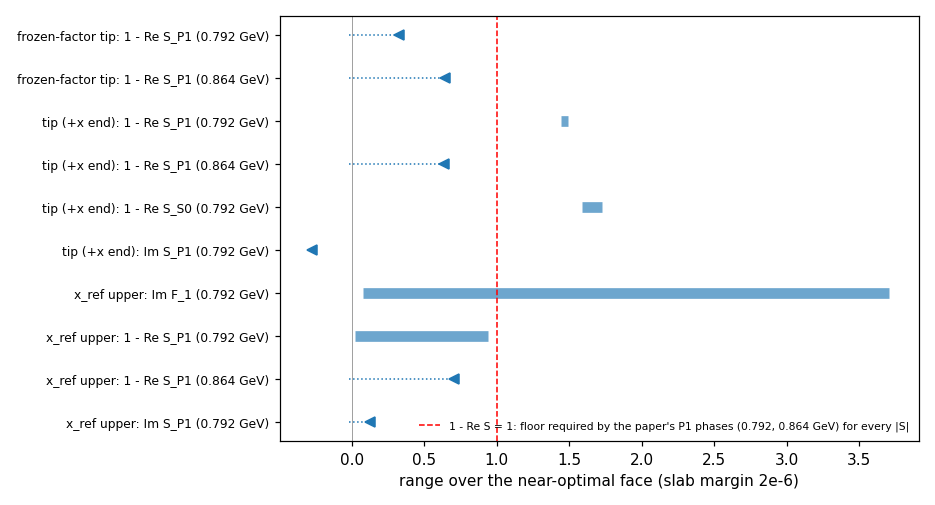
\includegraphics[width=0.85\textwidth]{figures/face_ranges.png}\caption{Ranges of the node functionals over the near-optimal faces: bars give $[\min,\max]$, triangles the maximum where only that was computed; the dashed line is the floor $1-\operatorname{Re}S=1$ that the phases of the paper require.}\end{figure}

\section{Questions}
We would be grateful for your help on the following points. They all concern the runs behind arXiv:2309.12402; we have read the code released with \fup\ and \cur, and are aware that several of these choices are made differently there.
\begin{enumerate}[leftmargin=*,itemsep=4pt]
\item In (3.73), which norm did you use for the sum-rule residuals, and is the QCD value compared with the raw moment $\int_4^{s_0}\rho(x)x^n\,dx$ or with the normalised one, divided by $s_0^{\,n+2}$ as in (2.56)? In our implementation a per-moment box of half-width $2\times10^{-3}$ on the raw moments is the only reading of $\epsilon^{SR}=2\times10^{-3}$ that is feasible.
\item In (3.75), is the factor between $F$ and $\mathcal F$ evaluated at each node $s_i>s_0$, or at $s_0$ for all of them? The two readings move the UV $+x$ end from 0.0760 to 0.0796 and change the shape of the P1 wave considerably.
\item Was a bound on the double spectral density $\rho_{ij}$, of the kind introduced in Section~3 of \meth\ or the $\ell^4$ bound used in \fupc, applied in these runs, and if so at what scale? Without such a bound the finite problem is ill-posed at 192-bit precision, and with our in-model rule the $+x$ ends of Figs.~3 and~4 agree with yours to 0.4\,\%.
\item For the three points of Figs.~9 and~10, were the plotted amplitudes the optimal points returned by the solver for the support problem, or was a saturation (Watson) step of the kind used in \cur\ already applied to select them? Our face diagnostic suggests that at the $x_{\rm ref}$ point the boundary alone does not fix the P1 wave.
\item If they are still available, the $(f_0^0(3),f_1^1(3))$ coordinates and $|S_{P1}(s)|$ of the red, pink and light pink points, together with the value of $s_0$ used for Figs.~8--11, would allow a direct comparison.
\end{enumerate}
We would be happy to share any of our solutions, the intermediate files or the full log of the runs.

\section*{References}
\begin{itemize}[leftmargin=*,itemsep=2pt]
\item Y.~He and M.~Kruczenski, \emph{Bootstrapping gauge theories}, \href{https://arxiv.org/abs/2309.12402}{arXiv:2309.12402} (the paper reproduced here).
\item Y.~He and M.~Kruczenski, \emph{Gauge Theory Bootstrap: Pion amplitudes and low energy parameters}, \href{https://arxiv.org/abs/2403.10772}{arXiv:2403.10772} (the follow-up paper; its released code was read, not run).
\item Y.~He and M.~Kruczenski, \emph{The Gauge Theory Bootstrap: Predicting pion dynamics from QCD}, \href{https://arxiv.org/abs/2505.19332}{arXiv:2505.19332} (current code of the repository \texttt{gauge-theory-bootstrap}).
\item Y.~He and M.~Kruczenski, \emph{S-matrix bootstrap in 3+1 dimensions: regularization and dual convex problem}, JHEP 08 (2021) 125, \href{https://arxiv.org/abs/2103.11484}{arXiv:2103.11484} (the earlier method paper whose Section~3 introduces the regularisation of the double spectral density).
\end{itemize}
\end{document}
